\documentclass[11pt,a4paper]{article}
\usepackage[margin=2.5cm]{geometry}
\usepackage{amsmath,amssymb,booktabs,graphicx,float}
\newcommand{\ii}{\mathrm{i}}
\newcommand{\uu}{\mathbf{u}}
\title{Phonon transmission across a loosely bonded crystal/metal interface:\\ derivation and implementation notes}
\author{I.~Israel\thanks{Replace with full name and affiliation.}}
\date{\today}
\begin{document}
\maketitle
\begin{abstract}
Technical note accompanying the code in this repository. It derives the reflection and transmission
amplitudes of plane elastic waves at a planar interface described by tangential and normal spring constants
(the loose-bond acoustic mismatch model of Every, Koos and Wolfe~\cite{Every1984}), the power coefficients,
the flux and Debye averages, and the closed-form limits used to validate the implementation.
\end{abstract}


This appendix derives the reflection and transmission amplitudes used in
the thesis chapter: the field expressions for each wave, the coefficient matrix of
the boundary-value problem, the SH channel, the power coefficients, and closed-form checks.

\section{Material parameters}

Table~\ref{tab:app_materials} lists the parameters entering the model. The Lam\'e parameters
for sapphire, Al, Nb and Ta are those of the thesis (Table~\ref{tab:app_materials} lists them); the velocities follow
from $V_T=\sqrt{\mu/\rho}$ and $V_L=\sqrt{(\lambda+2\mu)/\rho}$. Cu is not part of that
calculation and retains the values of Ref.~\cite{Every1984}.

\begin{table}[H]
\centering
\caption{Isotropic parameters used in the interface model.
Densities are assumed bulk values; Cu values are from Ref.~\cite{Every1984}.}
\label{tab:app_materials}
\begin{tabular}{lccccc}
\toprule
Material & $\lambda$ [GPa] & $\mu$ [GPa] & $\rho$ [kg\,m$^{-3}$] & $V_L$ [m/s] & $V_T$ [m/s]\\
\midrule
Sapphire & 139.8 & 166.24 & 3986  & 10885 & 6458\\
Al       & 58.7  & 26.2   & 2700  & 6415  & 3115\\
Nb       & 145   & 39.7   & 8570  & 5117  & 2152\\
Ta       & 149.3 & 70.55  & 16650 & 4176  & 2058\\
Cu       & 106.0 & 45.6   & 8930  & 4700  & 2260\\
\bottomrule
\end{tabular}
\end{table}

\section{Geometry, conventions and unknowns}

The interface is the plane $z=0$. The crystal (sapphire, subscript $c$) occupies $z<0$ and
the metal (subscript $m$) occupies $z>0$. The $x$ axis lies in the interface, and all fields
are independent of $y$. The time dependence is $e^{-\ii\omega t}$. Each medium is isotropic
with density $\rho$, wave speeds $V_L$, $V_T$ and Lam\'e constants
\begin{equation}
  \mu=\rho V_T^2,\qquad \lambda=\rho V_L^2-2\mu,\qquad \lambda+2\mu=\rho V_L^2 .
\end{equation}
Because $z$ points from the crystal into the metal, the incident and transmitted waves travel
towards $+z$ and the reflected waves towards $-z$. This is the opposite of the drawing in
Fig.~\ref{fig:angular}(a), which has the crystal on top, but the physics is
identical.

\section{Wave equation and Helmholtz potentials}

In each medium
\begin{equation}
  \rho\,\ddot{\uu}=(\lambda+2\mu)\nabla(\nabla\!\cdot\!\uu)-\mu\,\nabla\times\nabla\times\uu .
\end{equation}
For motion in the $x$--$z$ plane write
\begin{equation}
  \uu=\nabla\phi+\nabla\times(\psi\,\hat{\mathbf y}),\qquad
  \ddot\phi=V_L^2\nabla^2\phi,\qquad \ddot\psi=V_T^2\nabla^2\psi ,
\end{equation}
which gives $u_x=\partial_x\phi-\partial_z\psi$ and $u_z=\partial_z\phi+\partial_x\psi$.
The scalar $\phi$ carries the longitudinal (L) wave and $\psi$ the in-plane transverse (SV)
wave. The component $u_y$ (SH) is decoupled and treated in Sec.~\ref{app:SH}. The stress is
\begin{equation}
  \sigma_{ij}=\lambda\,\delta_{ij}\,\nabla\!\cdot\!\uu+\mu\,(\partial_iu_j+\partial_ju_i).
\end{equation}

\section{Plane waves, conserved slowness and Snell's law}

Take plane waves
\begin{equation}
  \phi=A\,e^{\ii\omega(px+s\,k_L z-t)},\qquad
  \psi=B\,e^{\ii\omega(px+s\,k_T z-t)} ,
\end{equation}
where $s=\pm1$ is the sign of the vertical propagation direction and $p$ is the horizontal
slowness. The boundary conditions must hold for every $x$ at $z=0$, so every wave of the
problem has the same $p$, which is Snell's law:
\begin{equation}
  p=\frac{\sin\theta_i}{V_i}=\frac{\sin\theta_j}{V_j}\quad\text{for every wave } j .
\end{equation}
Substituting into the wave equations gives the vertical slowness
\begin{equation}
  k_{j}(p)=\sqrt{V_j^{-2}-p^{2}}\,,\qquad \cos\theta_j=V_j\,k_j ,
  \label{eq:kz}
\end{equation}
for $j\in\{L,T\}$ in either medium. If $p>1/V_j$, then $k_j$ is purely imaginary. The branch
$\operatorname{Im}k_j\ge0$ is chosen, $k_j=\ii\sqrt{p^2-V_j^{-2}}$, so that the wave decays
away from the interface (it decays for $z\to+\infty$ with $s=+1$ and for $z\to-\infty$ with
$s=-1$). Such a wave is evanescent and carries no energy.

\section{Displacements and stresses of each wave}

Differentiating the plane waves gives, for an L wave,
\begin{align}
  u_x&=\ii\omega p\,A, & u_z&=\ii\omega s k_L A,\\
  \sigma_{xz}&=\mu(\partial_zu_x+\partial_xu_z)=-2\mu\,\omega^2\,s\,p\,k_L A,\\
  \sigma_{zz}&=\lambda\nabla\!\cdot\!\uu+2\mu\,\partial_zu_z
   =-\omega^2\Big(\tfrac{\lambda}{V_L^2}+2\mu k_L^2\Big)A
   =-\omega^2(\rho-2\mu p^2)A ,
\end{align}
where $\nabla\!\cdot\!\uu=\nabla^2\phi=-\omega^2A/V_L^2$ and
$\lambda/V_L^2+2\mu k_L^2=(\lambda+2\mu)/V_L^2-2\mu p^2=\rho-2\mu p^2$. For an SV wave,
$\nabla\!\cdot\!\uu=0$ and
\begin{align}
  u_x&=-\ii\omega s k_T B, & u_z&=\ii\omega p\,B,\\
  \sigma_{xz}&=\mu\omega^2(k_T^2-p^2)B=\omega^2(\rho-2\mu p^2)B,\\
  \sigma_{zz}&=2\mu\,\partial_zu_z=-2\mu\,\omega^2\,s\,p\,k_T B ,
\end{align}
where $\mu(k_T^2-p^2)=\rho-2\mu p^2$ was used. The combination
\begin{equation}
  D\equiv\rho-2\mu p^2=\rho\,(1-2V_T^2p^2)
\end{equation}
appears everywhere; for a transverse wave of angle $\theta$ it equals $\rho\cos2\theta$.

All fields scale as $\omega A$ (displacement) or $\omega^2A$ (stress). Defining the
\emph{reduced} fields $\tilde u=u/\omega$ and $\tilde\sigma=\sigma/\omega^2$, the frequency
drops out of every equation except through the bond stiffness (Sec.~\ref{app:BC}).
Table~\ref{tab:fields} lists the reduced field vectors
$(\tilde u_x,\tilde u_z,\tilde\sigma_{xz},\tilde\sigma_{zz})$ per unit potential amplitude.

\begin{table}[H]
\centering
\caption{Reduced field vectors per unit potential amplitude.
$D=\rho-2\mu p^2$ is evaluated with the density and shear modulus of the medium containing the wave.}
\label{tab:fields}
\begin{tabular}{lcccc}
\toprule
wave & $\tilde u_x$ & $\tilde u_z$ & $\tilde\sigma_{xz}$ & $\tilde\sigma_{zz}$\\
\midrule
L  & $\ii p$ & $\ii s k_L$ & $-2\mu s\,p\,k_L$ & $-D$\\
SV & $-\ii s k_T$ & $\ii p$ & $D$ & $-2\mu s\,p\,k_T$\\
\bottomrule
\end{tabular}
\end{table}

\section{Wave content of the problem}

An incident wave in the crystal (type L or SV, $s=+1$) generates a reflected L and a reflected
SV ($s=-1$) in the crystal, and a transmitted L and a transmitted SV ($s=+1$) in the metal.
Their potential amplitudes are
\begin{equation}
  \mathbf x=(A_{r},\,B_{r},\,A_{t},\,B_{t})^{\mathsf T}.
\end{equation}
The incident potential is normalised to unit displacement amplitude. For a propagating wave
$|\tilde u|^2=(p^2+k_j^2)|A|^2=|A|^2/V^2$, so $A_{\rm inc}=V_{\rm inc}$, and the amplitude
coefficients are
\begin{equation}
  \Gamma_{cL}=\frac{A_r}{V_{L,c}},\quad
  \Gamma_{cT}=\frac{B_r}{V_{T,c}},\quad
  \Gamma_{mL}=\frac{A_t}{V_{L,m}},\quad
  \Gamma_{mT}=\frac{B_t}{V_{T,m}} .
  \label{eq:Gamma}
\end{equation}
For propagating waves, $|\Gamma|$ is the displacement amplitude relative to the incident
one; for an evanescent wave, $\Gamma$ is only a rescaled potential amplitude.

\section{Boundary conditions}
\label{app:BC}

The interface is a layer of distributed springs with tangential stiffness $K_\parallel$ and
normal stiffness $K_\perp$ (stress per unit relative displacement). The conditions are
\begin{align}
  &\text{continuity of traction:} && \sigma^{c}_{xz}=\sigma^{m}_{xz},\qquad \sigma^{c}_{zz}=\sigma^{m}_{zz},
  \label{eq:BCtraction}\\
  &\text{spring law:} && \sigma^{c}_{xz}=K_\parallel\,(u^{m}_x-u^{c}_x),\qquad
  \sigma^{c}_{zz}=K_\perp\,(u^{m}_z-u^{c}_z),
  \label{eq:BCspring}
\end{align}
where the superscript denotes the total field (incident plus reflected for $c$; transmitted
for $m$) at $z=0$. The limits are
\begin{equation}
  K\to\infty:\ u^c=u^m\ \ (\text{welded}),\qquad
  K\to0:\ \sigma^c=0\ \ (\text{free surface; the metal decouples}).
\end{equation}
Dividing Eq.~\eqref{eq:BCspring} by $\omega^2$ and using $u=\omega\tilde u$ gives
$\tilde\sigma=(K/\omega)\,\Delta\tilde u$. The coupling is expressed through the dimensionless parameters
\begin{equation}
  \alpha_\parallel=\frac{K_\parallel}{\rho_cV_{T,c}\,\omega},\qquad
  \alpha_\perp=\frac{K_\perp}{\rho_cV_{L,c}\,\omega},
  \label{eq:alpha_omega}
\end{equation}
so that $\alpha\propto1/\omega$ for a frequency-independent stiffness. The reduced stiffnesses are
\begin{equation}
  \tilde K_\parallel=\frac{K_\parallel}{\omega}=\alpha_\parallel\,\rho_cV_{T,c}
  =\alpha_\parallel\frac{\mu_c}{V_{T,c}},
  \qquad
  \tilde K_\perp=\frac{K_\perp}{\omega}=\alpha_\perp\,\rho_cV_{L,c}
  =\alpha_\perp\frac{\lambda_c+2\mu_c}{V_{L,c}} .
  \label{eq:alpha_reduced}
\end{equation}

\section{The $4\times4$ linear system}

Write $\tilde\sigma^{w}$ and $\tilde u^{w}$ for the entries of Table~\ref{tab:fields} of wave
$w\in\{rL,rT,tL,tT,\mathrm{inc}\}$. Eq.~\eqref{eq:BCtraction} gives
\begin{align}
  \tilde\sigma_{xz}^{rL}A_r+\tilde\sigma_{xz}^{rT}B_r-\tilde\sigma_{xz}^{tL}A_t-\tilde\sigma_{xz}^{tT}B_t
   &=-\tilde\sigma_{xz}^{\rm inc},\\
  \tilde\sigma_{zz}^{rL}A_r+\tilde\sigma_{zz}^{rT}B_r-\tilde\sigma_{zz}^{tL}A_t-\tilde\sigma_{zz}^{tT}B_t
   &=-\tilde\sigma_{zz}^{\rm inc}.
\end{align}
Substituting $\tilde\sigma^c=\tilde\sigma^{\rm inc}+\tilde\sigma^{r}$ and
$\tilde u^c=\tilde u^{\rm inc}+\tilde u^{r}$ into Eq.~\eqref{eq:BCspring} gives, for the
tangential component,
\begin{equation}
  \big(\tilde\sigma_{xz}^{rL}+\tilde K_\parallel\tilde u_x^{rL}\big)A_r
  +\big(\tilde\sigma_{xz}^{rT}+\tilde K_\parallel\tilde u_x^{rT}\big)B_r
  -\tilde K_\parallel\tilde u_x^{tL}A_t-\tilde K_\parallel\tilde u_x^{tT}B_t
  =-\big(\tilde\sigma_{xz}^{\rm inc}+\tilde K_\parallel\tilde u_x^{\rm inc}\big),
\end{equation}
and the normal component is identical with $(x,xz,\parallel)\to(z,zz,\perp)$. In matrix form
$M\mathbf x=\mathbf b$ with
\begin{equation}
  M=\begin{pmatrix}
  \tilde\sigma_{xz}^{rL} & \tilde\sigma_{xz}^{rT} & -\tilde\sigma_{xz}^{tL} & -\tilde\sigma_{xz}^{tT}\\[2pt]
  \tilde\sigma_{zz}^{rL} & \tilde\sigma_{zz}^{rT} & -\tilde\sigma_{zz}^{tL} & -\tilde\sigma_{zz}^{tT}\\[2pt]
  \tilde\sigma_{xz}^{rL}+\tilde K_\parallel\tilde u_x^{rL} & \tilde\sigma_{xz}^{rT}+\tilde K_\parallel\tilde u_x^{rT} &
   -\tilde K_\parallel\tilde u_x^{tL} & -\tilde K_\parallel\tilde u_x^{tT}\\[2pt]
  \tilde\sigma_{zz}^{rL}+\tilde K_\perp\tilde u_z^{rL} & \tilde\sigma_{zz}^{rT}+\tilde K_\perp\tilde u_z^{rT} &
   -\tilde K_\perp\tilde u_z^{tL} & -\tilde K_\perp\tilde u_z^{tT}
  \end{pmatrix},\quad
  \mathbf b=-\begin{pmatrix}
  \tilde\sigma_{xz}^{\rm inc}\\ \tilde\sigma_{zz}^{\rm inc}\\
  \tilde\sigma_{xz}^{\rm inc}+\tilde K_\parallel\tilde u_x^{\rm inc}\\
  \tilde\sigma_{zz}^{\rm inc}+\tilde K_\perp\tilde u_z^{\rm inc}
  \end{pmatrix}.
\end{equation}
In the welded limit rows~3 and~4 are divided by $\tilde K$ and $\tilde K\to\infty$, giving
$\tilde u^{rL}_xA_r+\tilde u^{rT}_xB_r-\tilde u^{tL}_xA_t-\tilde u^{tT}_xB_t=-\tilde u^{\rm inc}_x$
and the same for $z$. The system has no useful closed form for general $\theta_i$; it is
solved numerically as a complex $4\times4$ system at each angle, and the amplitudes follow
from Eq.~\eqref{eq:Gamma}. Closed forms exist only in the special cases of
Sec.~\ref{app:checks}.

\section{SH waves}
\label{app:SH}

For polarisation along $y$, $u_y=C\,e^{\ii\omega(px+s k_Tz-t)}$ and the only relevant stress is
$\sigma_{yz}=\mu\,\partial_zu_y=\ii\omega\mu\,s\,k_T\,u_y$. The two conditions at $z=0$ are
continuity of $\sigma_{yz}$ and the spring law
$\sigma^{c}_{yz}=K_{SH}(u^m_y-u^c_y)$ with $\tilde K_{SH}=\alpha_{SH}\mu_c/V_{T,c}$. For unit
incident amplitude, reflected amplitude $R$ and transmitted amplitude $T_r$,
\begin{align}
  a(1-R)&=b\,T_r,\\
  \ii a(1-R)&=\tilde K_{SH}\,(T_r-1-R),
\end{align}
with $a=\mu_ck_{T,c}$ and $b=\mu_mk_{T,m}$. The solution is
\begin{equation}
  T_r=\frac{2}{\,1+b/a-\ii\,b/\tilde K_{SH}\,},\qquad R=1-\frac{b}{a}T_r .
  \label{eq:SHclosed}
\end{equation}
The model sets $\alpha_{SH}=\alpha_\parallel$, because SH motion is purely tangential
(an assumption of this model).

\section{Energy flux and power coefficients}

For a propagating plane wave with displacement amplitude $a$, the time-averaged energy
density is $\tfrac12\rho\omega^2|a|^2$. It travels at velocity $V$ along the propagation
direction, so its $z$-flux is $\langle P_z\rangle=\tfrac12\rho\,\omega^2|a|^2\,V\cos\theta$,
with $\cos\theta=Vk$ from Eq.~\eqref{eq:kz}. The fraction of the incident power carried by
the outgoing wave $j$ is therefore
\begin{equation}
  W_j=|\Gamma_j|^2\,\frac{\rho_jV_j\cos\theta_j}{\rho_{\rm inc}V_{\rm inc}\cos\theta_{\rm inc}}
  \ \ \text{(propagating)},\qquad W_j=0\ \ \text{(evanescent)}.
  \label{eq:W}
\end{equation}
Cross terms between different modes do not contribute, by modal power orthogonality in a
lossless medium (Auld, \emph{Acoustic Fields and Waves in Solids}, Vol.~II). The transmission
probability is $W_{\rm trans}=W_{mL}+W_{mT}$ and the reflection probability is
$W_{\rm refl}=W_{cL}+W_{cT}$.

\paragraph{Energy conservation.} The power flowing in $+z$ is
$-\tfrac12\operatorname{Re}[\sigma_{iz}\,v_i^{*}]$ with $v=-\ii\omega u$. Traction is
continuous, so with $\sigma\equiv\sigma^c=\sigma^m$,
\begin{equation}
  P^{c}_z-P^{m}_z=-\tfrac12\operatorname{Re}\!\big[\,\ii\omega\,\sigma_{iz}\,(u^c_i-u^m_i)^{*}\big]
   =\tfrac12\operatorname{Re}\!\big[\ii\omega\,K\,|\Delta u|^2\big]=0
\end{equation}
for real $K$ (using $\sigma=K\,\Delta u$, $\Delta u=u^m-u^c$, summed over $i=x,z$). A purely
elastic spring stores energy but dissipates none, so
$W_{cL}+W_{cT}+W_{mL}+W_{mT}=1$ at every angle. This was verified numerically to $10^{-8}$
for the welded and spring cases and for SH.

\section{Closed-form checks}
\label{app:checks}

\paragraph{Normal incidence.} With $p=0$ the L and SV problems decouple. For one wave type with
impedances $Z_c=\rho_cV_c$ and $Z_m=\rho_mV_m$, write
$u_c=e^{\ii k_cz}+Re^{-\ii k_cz}$ and $u_m=T e^{\ii k_mz}$. Then
$\sigma_c=\ii\omega Z_c(1-R)$ and $\sigma_m=\ii\omega Z_mT$. Continuity of traction gives
$Z_c(1-R)=Z_mT$, and the spring law with $K=\alpha Z_c\omega$ gives
$\ii Z_mT=\alpha Z_c(T-1-R)$. With $r=Z_m/Z_c$,
\begin{equation}
  T=\frac{2}{(1+r)-\ii\,r/\alpha},\qquad
  W_{\rm trans}=r|T|^2=\frac{4r}{(1+r)^2+r^2/\alpha^2}.
  \label{eq:normal_spring}
\end{equation}
For $\alpha\to\infty$ this is the acoustic-mismatch result $4r/(1+r)^2$. For sapphire/Ta
(transverse impedances $Z_c=2.57\times10^7$ and $Z_m=3.43\times10^7$ kg\,m$^{-2}$s$^{-1}$,
$r=1.33$) and $\alpha=1$ it gives $0.739$, which is the left end of the orange curve in
Fig.~\ref{fig:angular}(d).

\paragraph{Free surface ($K\to0$).} The metal decouples and rows~1 and~2 reduce to
$\sigma_{xz}^c=\sigma_{zz}^c=0$. With an incident SV wave $B_{\rm inc}=V_{T,c}$ and
$D=\rho_c\cos2\theta$,
\begin{align}
  2\mu p\,k_L\,A_r+D\,B_r&=-D\,B_{\rm inc},\\
  -D\,A_r+2\mu p\,k_T\,B_r&=2\mu p\,k_T\,B_{\rm inc}.
\end{align}
The determinant is $\Delta=4\mu^2p^2k_Lk_T+D^2$ (the Rayleigh-type denominator), and
\begin{equation}
  A_r=-\frac{4\mu p\,k_T\,D}{\Delta}B_{\rm inc},\qquad
  B_r=\frac{4\mu^2p^2k_Lk_T-D^2}{\Delta}B_{\rm inc}.
\end{equation}
With $\kappa=V_L/V_T$, $\sin\theta_L=\kappa\sin\theta$, $\mu pk_T=\tfrac12\rho\sin2\theta$ and
$\mu pk_L=\rho\sin2\theta_L/(2\kappa^2)$,
\begin{equation}
  \Gamma_{T\to L}=-\frac{\kappa\sin4\theta}{\sin2\theta\,\sin2\theta_L+\kappa^2\cos^2 2\theta},\qquad
  \Gamma_{T\to T}=\frac{\sin2\theta\,\sin2\theta_L-\kappa^2\cos^22\theta}{\sin2\theta\,\sin2\theta_L+\kappa^2\cos^22\theta}.
  \label{eq:freeTL}
\end{equation}

\section{Critical angle and the structure of Fig.~\ref{fig:angular}(c,d)}

For an incident SV wave, $p=\sin\theta/V_{T,c}$, and the reflected L wave in sapphire is
propagating only if $p<1/V_{L,c}$, that is
\begin{equation}
  \theta<\theta_c=\arcsin\frac{V_{T,c}}{V_{L,c}}=36.4^\circ .
\end{equation}
At $\theta_c$ the reflected L wave grazes the surface ($\cos\theta_L=0$,
$\sin2\theta_L=0$); above $\theta_c$ it is evanescent and $\sin2\theta_L$ becomes imaginary in
Eq.~\eqref{eq:freeTL}. At $\theta_c$ the free-surface amplitude is finite:
\begin{equation}
  |\Gamma_{T\to L}|^2_{\theta_c}=\left(\frac{\sin4\theta_c}{\kappa\cos^22\theta_c}\right)^{2}=14.7 .
\end{equation}
The peak is a cusp from the square-root branch point of $k_L$, not a divergence; on a finite
angular grid the plotted maximum is slightly lower because the grid does not land exactly on
$\theta_c$.

The quantity in panel~(c) is a \emph{displacement amplitude} squared, not a power, so it can
exceed one without violating energy conservation: the associated power is
$W_{cL}=|\Gamma_{T\to L}|^2\,\kappa\cos\theta_L/\cos\theta$ from Eq.~\eqref{eq:W}, which goes
to zero at $\theta_c$. For SV incidence the metal waves are always propagating because
sapphire is the fast medium: for Ta, $p_{\max}=1/V_{T,c}=0.155$~s/km is below
$1/V_{L,m}=0.239$~s/km and $1/V_{T,m}=0.486$~s/km. The cusp in panel~(d) is the transmission
side of the same branch point.

\section{Angular and Debye averages}

For isotropic phonon incidence from the crystal, the number flux per solid angle is
proportional to $\cos\theta$, so the flux-weighted transmission of a mode is
\begin{equation}
  \langle W\rangle_\nu=\frac{\int_0^{\pi/2}W_\nu(\theta)\cos\theta\sin\theta\,d\theta}
                          {\int_0^{\pi/2}\cos\theta\sin\theta\,d\theta}
   =2\int_0^{\pi/2}W_\nu(\theta)\cos\theta\sin\theta\,d\theta ,
\end{equation}
with $\nu\in\{\mathrm{L,SV,SH}\}$ and $W_\nu$ the transmission probability for an incident wave
of type $\nu$ ($W_{\rm trans}$ from Sec.~\ref{app:SH} for SH). The average over the two
transverse polarisations is $\langle W\rangle_T=\tfrac12(\langle W\rangle_{SV}+\langle W\rangle_{SH})$.
Weighting by the Debye density of states, $\propto V^{-3}$ per mode (one L and two T), gives
\begin{equation}
  \langle W\rangle_{\rm Debye}
  =\frac{2V_{T,c}^{-3}\langle W\rangle_T+V_{L,c}^{-3}\langle W\rangle_L}{2V_{T,c}^{-3}+V_{L,c}^{-3}} .
\end{equation}
The frequency enters only through $\alpha\propto1/\omega$ (Eq.~\eqref{eq:alpha_omega}). The
relation between $\alpha$ and phonon energy in Fig.~\ref{fig:vs_alpha}
($\alpha=1$ at $2.48$~meV, $K$ frequency independent) is an assumption, not a result of the
model.

\section{Figures}
\begin{figure}[H]\centering
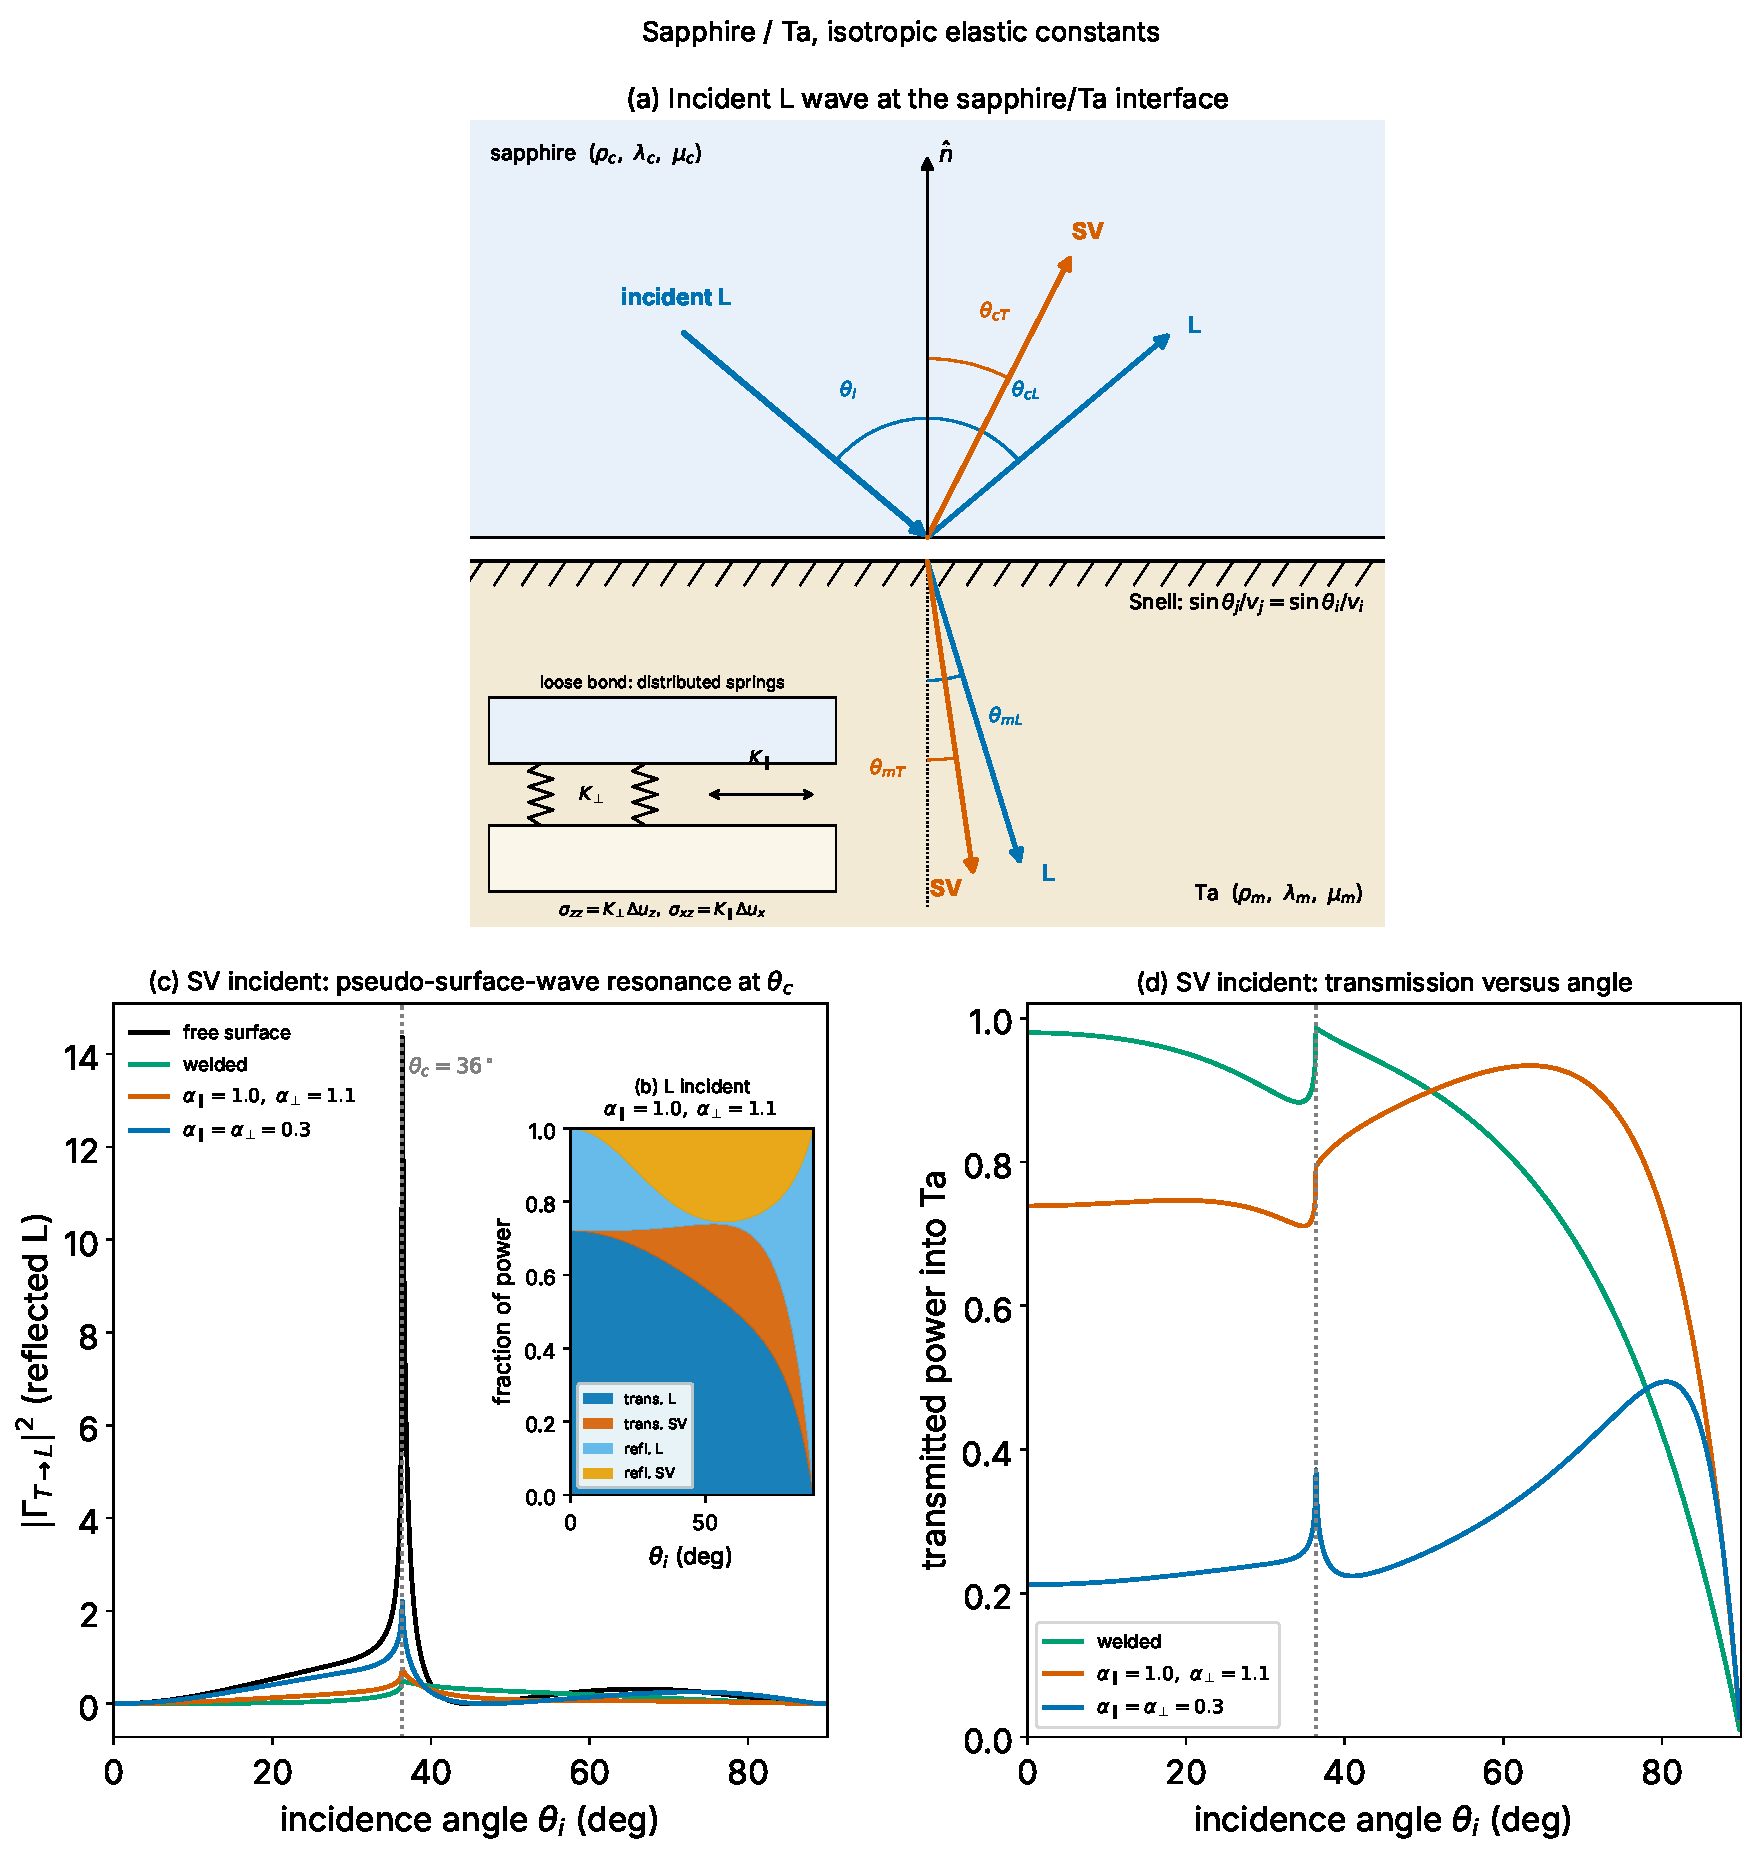
\includegraphics[width=0.95\textwidth]{../figures/interface_angular.pdf}
\caption{Sapphire/Ta interface: (a) ray diagram with the loose-bond boundary condition; (b) power partition of an incident L wave; (c) reflected-L amplitude for an incident SV wave; (d) power transmitted into Ta for an incident SV wave.}
\label{fig:angular}
\end{figure}
\begin{figure}[H]\centering
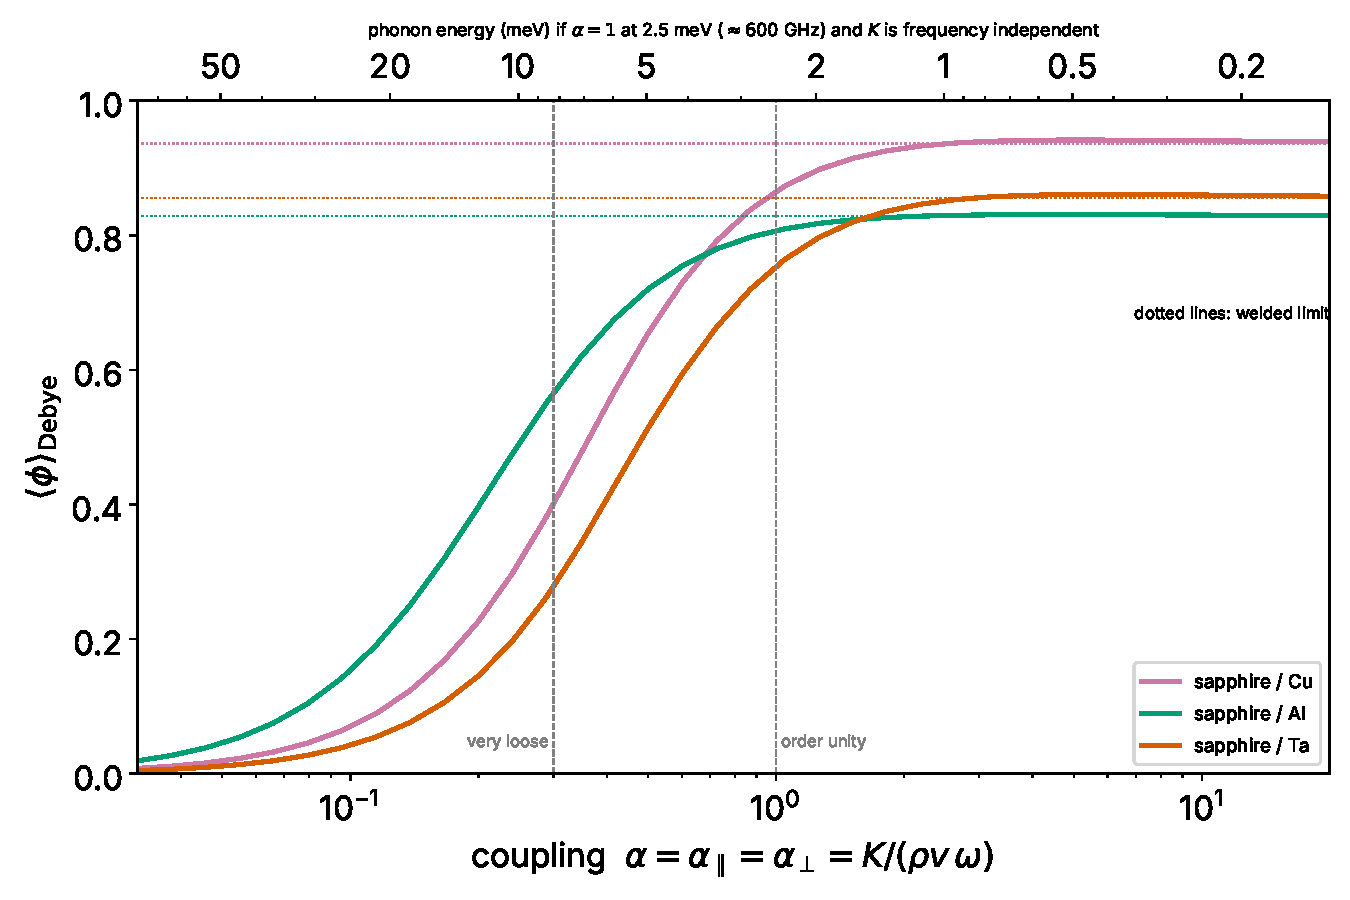
\includegraphics[width=0.8\textwidth]{../figures/interface_vs_alpha.pdf}
\caption{Debye- and flux-averaged transmission probability versus coupling $\alpha=\alpha_\parallel=\alpha_\perp$.}
\label{fig:vs_alpha}
\end{figure}
\begin{thebibliography}{9}
\bibitem{Every1984} A.~G. Every, G.~L. Koos and J.~P. Wolfe, Phys. Rev. B \textbf{29}, 2190 (1984).
\bibitem{Kaplan1979} S.~B. Kaplan, J. Low Temp. Phys. \textbf{37}, 343 (1979).
\bibitem{Auld1973} B.~A. Auld, \emph{Acoustic Fields and Waves in Solids}, Vol.~II (Wiley, 1973).
\end{thebibliography}
\end{document}
